We have designed and implemented a Jupyter kernel for MMT.
We describe its interface in Section~\ref{sec:kernel:syntax} and the implementation in Section~\ref{sec:kernel:impl}.

\subsection{Interface}\label{sec:kernel:syntax}

MMT differs from typical computational engines in Jupyter in that it does not only or even primarily perform computation but also handles symbolic expressions with uninterpreted function symbols. \begin{newpart}{MK@FR: correct and elaborate; I think this is an important issue here} Another important difference is how MMT handles context and background. Normal computational engines build and maintain a dynamic context of declarations with imperative assignment  or functional (stack-oriented) shadowing and rely on an -- often object-oriented -- background library of computational functionality. MMT is based on theory graphs for both context and background knowledge management. 
\end{newpart}
To adequately handle these subtleties, we systematically specified a new interface for interacting with MMT in Jupyter-style.  

\paragraph{Input}
The possible inputs excepted by the MMT kernel are divided into three groups.
\begin{itemize}
\item \textbf{Global management commands} allow displaying and deleting all current sessions.
 In practice, these commands are typically not available to users, which should only have access to their own session.
\item \textbf{Local management commands} allow starting, quitting, and restarting the current session. These are the main commands issued by the frontend in response to user action.
\item \textbf{Content commands} are the mathematically relevant commands and described below.
\end{itemize}

The content commands are divided into two groups:
\begin{itemize}
 \item \textbf{Write-commands} send new content to the backend in order to build MMT documents step by step.
   The backend maintains one implicit, ephemeral MMT document for each session, and any write command changes that document.
 \item \textbf{Read-commands} retrieve information from the backend without changing the session's document.
   These include lookups (both in the session document and in any other accessible document) or computations.
\end{itemize}

A write-command typically consists of a single MMT declaration roughly corresponding to a line in a typical MMT source file.
However, the nesting of declarations is very important in MMT (contrary to many programming language kernels where nesting is optional).\ednote{MK@FR: pick up the newpart from above.}
Therefore, all declarations that may contain other declarations (most importantly all MMT documents and theories) are split into parts as follows: the theory header, the list of nested declarations, and a special end-of-nesting marker. These are communicated in separate write-commands.
The MMT kernel maintains the current scope as an MMT URI of an MMT document or theory and updates it on every write-commands that opens or closes one of them.
This ensures that all nested declarations are parsed and interpreted in the right scope.

For example, the sequence of commands \ednote{@Kai: make this prettier and sync it with the example for which you add a screenshot later} on the left of Figure~\ref{fig:test_theory} builds two nested theories: the inner one refers to a type declared in the outer one. Figure~\ref{fig:test_theory} shows the equivalent in MMT surface syntax on the right. This corresponds to the ephemeral MMT document maintained by the MMT kernel.
\begin{figure}[ht]\centering
\begin{minipage}[c]{10cm}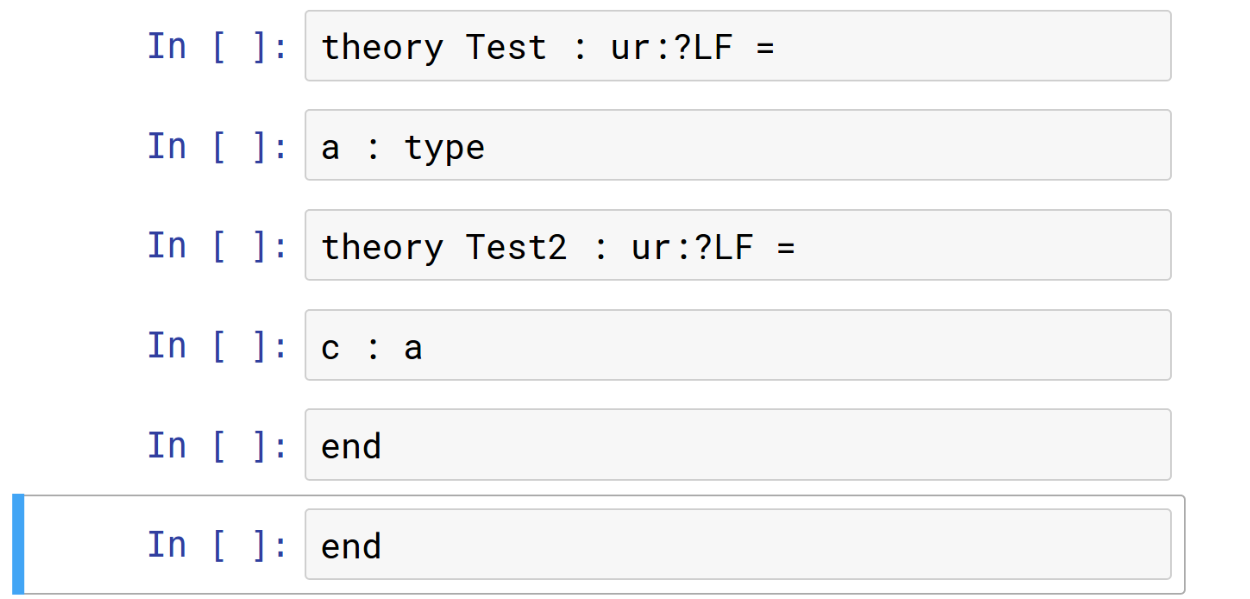
\includegraphics[width=10cm]{test_theory_jupyter}\end{minipage}
\begin{minipage}[c]{5cm}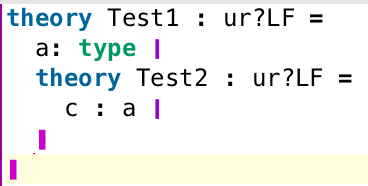
\includegraphics[width=5cm]{test_theory}\end{minipage}
\caption{Content Commands for Building Theory Graphs}\label{fig:test_theory}
\end{figure}

A special write-command is \texttt{eval T}.
It interprets \texttt{T} in the current scope, infers it type \texttt{A}, computes it, and then adds the declaration \texttt{resI:A=T} to the current theory, where \texttt{I} is a running counter of unnamed declarations.
This corresponds most closely to the REPL functionality in typical Jupyter kernels.

While write-commands correspond closely to the available types of MMT declarations, the set of read-commands is extensible.
For example, the commands \texttt{get U} where \texttt{U} is any MMT URI returns the MMT declaration of that URI.

\paragraph{Output}
The kernel returns the following kinds of return messages:
\begin{itemize}
\item \textbf{Admin messages} are strings returned in response to session management commands.
\item \textbf{New-element messages} return the declaration that was added by a write-command.
\item \textbf{Existing-element messages} return the declaration that was retrieved by a \texttt{get} command.
\end{itemize}
Like read-commands, the set of output messages is extensible.

The new-element and existing-element messages initially return the declaration in MMT's abstract syntax.
And a post-processing layer specific to Jupyter renders them in HTML+MathML presentation.
That way the core kernel functionality can be reused easily in other frontends.

\subsection{Implementation}\label{sec:kernel:impl}

\paragraph{Overview}
Our implementation consists of three layers.
The top layer is a Python module implements the abstract class for Jupyter kernels.
The bottom layer is a general-purpose MMT REPL handles all intelligence of MMT documents.
This can be reused easily in other frontends.
The two are connected by a thin middle layer that handles the communication between the other two.
Its main purpose is to format results in HTML and add interactive functionality via widgets.

The Jupyter infrastructure heavily relies on Python, especially when it comes to Jupyter widgets.
Therefore, it makes sense to implement our kernel in Python.
However, actually executing the user's commands requires a strong integration with the MMT implementation, which uses Scala.
That made it advisable to implement all Jupyter-specific functionality, especially the communication and management, in Python, while all mathematically relevant intelligence is handled in Scala.

This separation of programming languages is a generally difficult problem.
After some experiments with different solutions (e.g., HTTP communication) and discussion within the OpenDreamKit community, we identified the Py4j library~\cite{Py4j}\ednote{MK@KA: make a bibTeX entry in local.bib} as the best choice.
This is a Python-JVM bridge that allows seamless interaction between Python and any language (such as Scala) that compiles to the JVM.
Thus, our Python kernel can call MMT code directly.
Valuable Py4j features include callbacks from MMT to Python, shared memory (by treating pointers to JVM objects as Python values), and synchronized garbage collection.
That makes our kernel very robust against bit rot and allows benefiting from future improvements to the MMT backend.

Py4j is only JVM-specific, not Scala-specific.
That means that some Scala-specific constructs are not readily exposed to Python.
For example, both Python and Scala allow magic methods for treating any object as a function, but the JVM does not; moreover, the magic method is called \texttt{\_\_call\_\_} in Python and \texttt{apply} in Scala.
Similarly, Scala collections like lists are not automatically seen as their counterparts in Python.
Therefore, we wrote a Python module (which is distributed with MMT) that performs the bureaucracy of matching up advanced Python and Scala features.\ednote{MK@KA: can we point to this in the MMT code?}

\paragraph{Basic Functionality}\ednote{MK@KA/FR: write something here or remove paragraph heading.}

\ednote{KA: I just had these two sections written, and pasted them here so they might not fit perfectly}

\subsection{Communication Protocol}

Here we will give a higher-level overview of how communication between Jupyter frontend, kernel and MMT-backend takes place.
A more detailed low-level description of the protocol between the kernel and MMT backend is provided in the next section\ednote{MK: the stuff in 2.3.1 is mostly redundant now; probably completely eliminate the subsecti}. If you are interested in an explicit description of communication between the Jupyter frontend and the kernel please refer to the \hyperlink{https://jupyter-client.readthedocs.io/en/latest/messaging.html}{Messaging} section of the \hyperlink{http://jupyter.org/documentation}{Jupyter documentation}.\ednote{MK@KA: use citations here cite[section...][JupDoc]: make a bibTeX entry in local.bib}
Since a REPL always start with user a input, let us comply to that and start at the Jupyter frontend: the notebook.
Here the user inputs code which is then sent to our Jupyter kernel.
The kernel then forwards this input to MMT which evaluates it and sends the result back through the kernel to the frontend, which then displays said result.

\begin{figure}[ht]\centering
  \fbox{Active Computation Screenshot}
  \caption{Active Computation in Notebooks}\label{fig:active-computation}
\end{figure}

As we want present to visually powerful and interactive information to the user, we of course want to support the usage of Jupyter widgets in notebook output:
They serve as an ideal GUI library, by providing visually appealing, interactive and highly customizable GUI building blocks, see Figure~\ref{fig:active-computation}\ednote{KA: show active computation screenshot}, which shows a simple active computation example.
Therefore we have to extend our communication protocol to comply with the widget standards. So apart from the ususal plain text or HTML messages, we also have to support \textbf{widget messages}: these are commands to the kernel to open, modify, display a widget or register MMT functionalities to it.

In the active computation example the shown in Figure~\ref{fig:active-computation}, the ``Compute'' button is a widget that triggers a functionality in MMT which computes the variable, chosen with the selection button widget, by using the values provided by the number widgets. Realizing this coupling of widgets and MMT functionality requires a special interface between the kernel and the MMT backend, which is covered in the next section.
\ednote{KA: make pretty Diagramm to show what happens when e.g. buttons are clicked}



\begin{oldpart}{MK: mostly already said above. Probabely integrate what is not above an d eliminate this subsubsection}
  \subsubsection{Communication between Kernel and MMT Backend}
Although communication between the Jupyter-Kernel and MMT via HTTP would suffice for basic messages, containing plaintext or HTML, it proves exceedingly difficult to realize the integration of Jupyter widgets, where we have to be able to bidirectionally send object references between the kernel and the backend. During development it proved that the \hyperlink{https://www.py4j.org/}{Py4J} Python-Java-bridge, lets us overcome the issues we have, when communicating via HTTP and makes code more modular and easier to understand, on both Python and Scala side. As for all communication protocols, our main goal by using the Py4J-bridge is to create an interface between the MMT backend, which is implemented in Scala, and our Jupyter kernel, which is implemented in Python. This interface is created by providing an abstract class in Scala that features our desired methods. The actual implementation of these methods is done in a Python class, that can be transformed into a Java Class by using a special Py4J annotation. Since instantiation can only take place on the Python side, we need to send the thereby resulting object across the bridge to Scala. This can be done by providing the Python side with an entry point to the Java Virtual Machine (JVM) of our Scala backend, by starting a Py4JGateway-server there. When we now call a method of the converted Python object in Scala, we actually execute the Python code and get the result back in Scala. This mechanism allows us to conveniently register Scala callbacks to the Jupyter widgets, that enable them to interact with each other and the user alike and is therefore essential to using the full potential of the Jupyter widgets.

\ednote{@Kai: add a few details about how the communication works; e.g., by describing how one of the commands from the previous section is handled}
\end{oldpart}

\paragraph{Jupyter/MMT Widgets}
The use of a Python-JVM bridge pays off in particular when it allows us to reuse the widget library that is already part of the Python codebase of Jupyter.
It allows the top layer to call the middle layer in a way that passes the Python-based kernel environment of the top layer.\ednote{A small architecture diagram (e.g. in a wrapfigure) would be very helpful here.}
That way, the Scala-based middle layer can perform callbacks to the widget library.
Thus, the middle layer can choose to present some of the messages returned by the bottom layer as interactive HTML using widgets.

For example, when presenting a parametric theory as HTML+MathM, we can add a text input field next to every parameter.
Whenever the strings in these fields change, the frontend notifies the top layer, which passes on the change to the middle layer.
The middle layer then parses these strings and substitutes them in the body of the resulting declaration.
This is similar to but more general than the typical Jupyter functionality of rerunning a notebook when an input cell changes: while Jupyter uses a list of input cells and any change affects all subsequent cells, our widget amounts to a three structure in which input fields have local, nested scope.

\ednote{@Kai: this is a simple application that we might not finish by the deliverable deadline but that you should implement nonetheless. Stay in touch with me on the details. KA: for this we would probably need a custom widget}


\begin{newpart}{MK: just made this up from the screenshot (which I have cropped); move somewhere appropriate}
  \paragraph{In-Document Computation via Jupyter/MMT Widgets}
  Figure~\ref{fig:ac}\ednote{MK@KA: save much much more horizontal space (smaller browser window, so that it becomes believable that we embed this into a document.)} shows an example where a Jupyter/MMT widgets are used for in-document computation as specified D4.9~\cite{ODK-D4.9}.
  In fact the custom user interface shown there was simply assembled from simple Jupyter/MMT widgets.\ednote{MK@KA/FR: describe how they work instantiated to this specific example}
  This design makes constructing such interfaces much easier and the interaction functionalities much more powerful -- we still have the full power of a computational kernel in Jupyter at our fingertips. 
  To achive full document/notebook integration, as envisioned in D4.2~\cite{ODK-D4.2}, we only have to embed this notebook interface into the HTML5 presentation of the outer documnet (the one that contains the equation $E=mc^2$) and feed the document context information into the interior notebook as described in~\cite{ODK-D4.9} (this part of the integration can be re-used directly).
  \ednote{MK@KA/FR: For the evaluation (and Kai's thesis) we should make an sTeX document that contains $E=mc^2$ (e.g. by copying parts of \texttt{https://en.wikipedia.org/wiki/Mass-energy\_equivalence}) and really implement the in-document computation example. This would make a wonderful demo in Brussels.}

  \begin{figure}[ht]\centering
    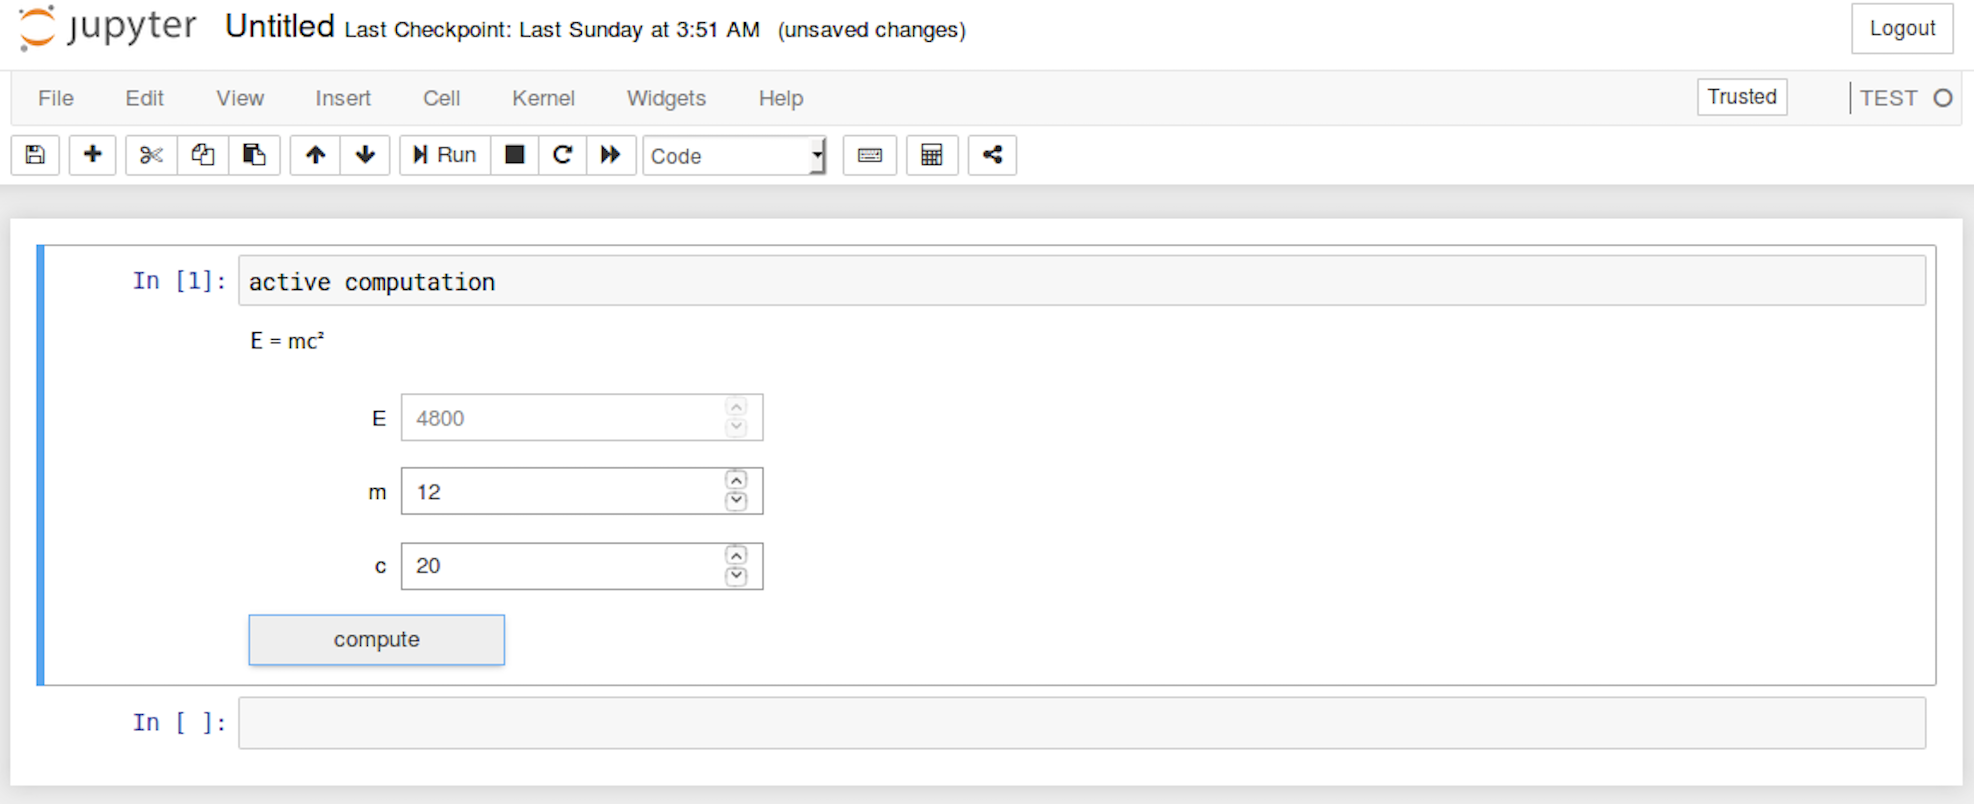
\includegraphics[width=12cm]{activecomp}
    \caption{Active Computation in Jupyter Notebooks via Jupyter/MMT Widgets}\label{fig:ac}
  \end{figure}
\end{newpart}

%%% Local Variables:
%%% mode: latex
%%% mode: visual-line
%%% fill-column: 5000
%%% TeX-master: "report"
%%% End:

%  LocalWords:  Jupyter newpart textbf ednote centering texttt includegraphics synchronized customizable inparaenum Realizing subsubsection
